%versi 2 (8-10-2016)
\chapter{Landasan Teori}
\label{chap:landasan teori}

Pada bab ini akan dijelaskan mengenai dasar teori yang digunakan sebagai acuan dalam mengembangkan perangkat lunak yang akan dibangun. Bab ini antara lain akan menjelaskan tentang sistem rekomendasi, \textit{cluster}, \textit{Library} PHP, dan Universitas Katolik Parahyangan.

\section{Sistem Rekomendasi}
\label{sec:sistem rekomendasi}

Sistem rekomendasi \cite{buku:sistem:rekomendasi} adalah alat dan teknik perangkat lunak yang menyediakan saran untuk item yang akan digunakan oleh pengguna. Rekomendasi tersebut berkaitan dengan penentuan keputusan seperti produk apa yang ingin dibeli, musik apa yang akan didengarkan, atau berita apa yang akan dibaca. Pengembangan sistem rekomendasi \cite{buku:sistem:rekomendasi} diawali dari pengamatan sederhana berupa rekomendasi yang diberikan oleh orang lain dalam membuat keputusan dalam kehidupan sehari-hari. Sistem rekomendasi ditujukan untuk individu atau personal yang kurang memiliki pengalaman pribadi. Contoh \textit{website} yang menggunakan sistem rekomendasi adalah Amazon.com. Sistem rekomendasi pada Amazon.com digunakan untuk mempersonalisasi toko \textit{online} untuk setiap pengguna. Karena dipersonalisasi hasil akan berbeda untuk pengguna yang berbeda. Item yang ditawarkan merupakan daftar item peringkat. Sistem rekomendasi mencoba memprediksi produk dengan cara mengumpulkan referensi dari pengguna lainnya.

% kemungkinan besar dihapus (ga kepake di skripsi, cuman informasi aja)
\subsection{Fungsi Sistem Rekomendasi}
Berikut merupakan fungsi dari sistem rekomendasi \cite{buku:sistem:rekomendasi} :
	\begin{enumerate}
		\item Meningkatkan jumlah penjualan barang\\
			Meningkatkan jumlah penjualan barang adalah fungsi yang paling penting untuk sistem rekomendasi komersial. Peningkatan jumlah penjualan item ini disebabkan karena penjualan item dilakukan tepat sasaran kepada pembeli yang memang membutuhkan dan menginginkan item tersebut. Tujuan ini tercapai karena barang yang direkomendasikan cenderung sesuai dengan kebutuhan dan keinginan pengguna.
			
		\item Menjual barang-barang yang lebih beragam\\
			Fungsi sistem rekomendasi lainnya adalah memungkinkan pengguna untuk memilih item yang mungkin sulit ditemukan tanpa rekomendasi yang tepat. Sistem rekomendasi akan merekomendasikan item yang tidak populer kepada pengguna yang tepat.
			
		\item Meningkatkan kepuasan pengguna\\
			Sistem rekomendasi yang dirancang dengan baik memberikan rekomendasi yang sesuai dengan kebutuhan pengguna sehingga pengguna akan merasa senang menggunakan sistem tersebut.
		
		\item Meningkatkan kesetiaan pengguna\\
			Pengguna akan tetap menggunakan sebuah \textit{website} jika sistem rekomendasi yang hasilkan rekomendasi yang sesuai dengan kebutuhan pengguna. 
			
		\item Lebih mengerti apa yang diinginkan pengguna\\
			Sistem dapat memebrikan hasil rekomendasi item yang sesuai dengan kebutuhan pengguna.
	\end{enumerate} \leavevmode

\subsection{Sumber Data dan Pengetahuan}
\label{sec:sumber data dan pengetahuan}
Sistem rekomendasi adalah sistem pemrosesan informasi yang secara aktif mengumpulkan berbagai jenis data untuk membangun rekomendasinya. Data utama berupa data item yang disarankan dan pengguna yang akan menerima rekomendasi. Data yang digunakan sistem rekomendasi mencakup pada tige jenis objek \cite{buku:sistem:rekomendasi}, yaitu :
	\begin{enumerate}
	\item \textbf{Item}\\
		Item adalah objek yang direkomendasikan, item bisa ditandai oleh kompleksitasnya dan nilai atau kegunaannya. Bisa bernilai positif jika sesuai atau negatif jika tidak sesuai dan pengguna membuat keputusan yang salah ketika memilih item dengan nilai negatif. Saat pengguna memperoleh item, pengguna akan dikenai \textit{cost}, berupa \textit{cognitive cost} untuk pencarian item tersebut dan \textit{the real monetary cost} yang dibayarkan untuk item tersebut.
		
		Sebagai contoh, perancangan sistem rekomendasi berita harus memperhitungkan kompelsitas item berita, Seperti struktur, representasi tekstual, dan kepentingan waktu yang bergantingan pada setiap item berita. Tetapi, pada saat yang sama, perancangan sistem rekomendasi harus memahami bahwa meskipun pengguna tidak membayar untuk membaca berita, selalu ada \textit{cognitive cost} yang terkait dengan mencari dan membaca item berita. Jika item yang dipilih relevan untuk pengguna, \textit{cost} didominasikan oleh manfaat memperoleh informasi yang berguna, jika item tidak relevan, nilai item untuk pengguna dan rekomendasinya negatif. Di domain lain, misalnya mobil atau investasi keuangan, \textit{the real monetary cost} dari item menjadi elemen penting untuk dipertimbangkan ketika memilih pendekatan rekomendasi yang paling tepat.
		
		Item dapat dikelompokkan menjadi dua kelompok, yaitu : item dengan kompleksitas dan nilai rendah dan item dengan kompleksitas dan nilai tinggi. Contoh dari item dengan kompleksitas dan nilai rendah adalah berita, halaman web, CD, dan film, sedangkan contoh untuk item dengan kompleksitas dan nilai tinggi adalah kamera digital, ponsel, PC, dll. Item paling kompleks yang telah dipertimbangkan adalah kebijakan asuransi, investasi keuangan, perjalanan, dan pekerjaan.
		
		Sistem rekomendasi dapat menggunakan berbagai properti dan fitur dari item yang digunakan. Misalnya pada sistem rekomendasi film  genre, sutradara, dan aktor dapat digunakan untuk menggambarkan film dan mempelajari bagaimana kegunaan suatu item berdasarkan fitur-fitur yang dimiliki item tersebut. Item dapat dipresentasikan menggunakan berbagai informasi dan pendekatan representasi, misalnya dalam cara meminimalis sebagai kode id tunggal atau dalam bentuk kumpulan atribut.
	
	\item \textbf{Pengguna}\\
		Pengguna adalah objek yang menggunakan sistem, memiliki tujuan dan karakteristik beragam. Untuk mempersonalisasi rekomendasi dan interaksi manusia komputer, sistem rekomendasi menggunakan berbagai informasi mengenai pengguna. Informasi ini dapat disusun dengan berbagai cara dan pemilihan informasi apa yang digunakan tergantung pada teknik rekomendasi yang digunakan.
		
		Sebagai contoh, dalam \textit{collaborative filtering} pengguna dimodelkan sebagai daftar sederhana yang berisikan peringkat yang disediakan oleh pengguna untuk beberapa item. Dalam sistem rekomendasi demografis, atribut sosiodemografi seperti usia, jenis kelamin, profesi, dan pendidikan akan digunakan. Data pengguna disebut model pengguna. Model pengguna berfungsi untuk mengkodekan preferensi dan kebutuhan. Sistem rekomendasi menghasilkan rekomendasi dengan membangun dan menggunakan model pengguna. Karena tidak ada sistem rekomendasi yang dipersonalisasi tanpa menggunakan model pengguna, kecuali sistem rekomendasi yang dibangun bukan sistem yang dipernonalisasi, seperti pemilihan \textit{top}-10.
		
		Pengguna juga dapat dijelaskan menggunakan data pola perilaku sperti pola penelusuran web atau pola pencarian perjalanan. Selain itu, data pengguna dapat mencakup hubungan antar pengguna seperti tingkat kepercayaan hubungan antara pengguna. Sistem rekomendasi munngkin menggunakan informasi ini untuk merekomendasikan item kepada pengguna yang memiliki selera serupa.
	
	\item \textbf{Transaksi}\\
		Transaksi adalah interaksi yang direkam antara pengguna sistem rekomendasi. Transaksi adalah data seperti log yang menyimpan informasi penting yang dihasilkan selama interaksi manusia komputer dan berguna untuk algoritma pembuatan rekomendasi yang digunakan sistem. Misalnya, log transaksi dapat berisi referensi ke item yang dipilih oleh pengguna dan deksripsi konteks seperti tujuan atau \textit{query} untuk rekomendasi tersebut. 
		
		Faktanya, peringkat adalah bentuk data transaksi paling populer yang dikumpulkan oleh sistem rekomendasi. Peringkat ini dapat dikumpulkan secara eksplisit atau implisit. Dalam kumpulan peringkat eksplisit, pengguna diminta untuk memberikan pendapatnya tentang suatu item menggunakan skala. Berikut merupakan bentuk dari peringkat yang populer di sistem rekomendasi :
		
		\begin{itemize}
			\item Peringkat numerik seperti bintang 1 - 5 seperti yang disediakan oleh Amazon.com.
		
			\item Peringkat ordinal seperti sangat setuju, setuju, netral, tidak setuju, dan sangat tidak setuju, dimana pengguna diminta untuk memilih diantara kelima peringkat tersebut yang menunjukkan pendapatnya menganai suatu item.
		
			\item Peringkat biner yang memodelkan pilihan dimana pengguna hanya diminta untuk memutuskan apakah suatu barang tersebut baik atau buruk.
		
			\item Peringkat unary dapat menunjukkan bahwa pengguna telah mengamati atau membeli suatu item atau menilai item secara positif.
		\end{itemize}
		
		Berdasarkan \cite{buku:sistem:rekomendasi:2}, Di antara alternatif yang ada untuk mengumpulkan pendapat pengguna, meminta peringkat item eksplisit adalah yang paling tepat. Masalah utama dalam peringkat eksplisit pengguna tidak bersedia memberikan peringkat selama nilainya tidak mudah dilihat, hal ini dapat menyebabkan peringkat yang tersedia terlalu sedikit, sehingga dapat menghasilkan kualitas rekomendasi yang buruk.
		
	\end{enumerate}
	
\subsection{Teknik Rekomendasi}
\label{teknik rekomendasi}
Berikut adalah teknik-teknik yang dapat digunakan pada sistem rekomendasi \cite{buku:sistem:rekomendasi}: %RS hanbook

\begin{enumerate}
	\item \textit{Content-based}\\
		Sistem merekomendasikan item yang mirip berdasarkan item yang disukai pengguna di masa lalu. Kesamaan dihitung berdasarkan fitur(atribut) yang terkait dengan item. misal , review positif film komedi, maka akan direkomendasikan film di genre yang sama. 

	\item \textit{Collaborative Filtering} \\
		 Rekomendasi berdasarkan item yang disukai pengguna lain yang memiliki kesamaan. Implementasi paling sederhana, merekomendasikan item yang disukai pengguna lain dengan selera serupa di masa lalu.  \textit{Collaborative Filtering} populer dan banyak digunakan pada sistem rekomendasi. \textit{Nearest neighbors} meningkatkan popularitas karena sederhana, efisien, dan kemampuan mereka untuk menghasilkan rekomendasi yang akurat dan menunjukkan ciri personal tertentu.
	
	\item \textit{Demographic} \\
		Rekomendasi berdasarkan profil demografis pengguna. Asumsinya bahwa rekomendasi yang berbeda harus dihasilkan untuk demografis yang berbeda. Misalnya diarahkan ke web dengan bahasa atau negara pengguna. 

	\item \textit{Knowledge-based} \\
		Merekomendasikan item berdasarkan pengetahuan domain spesifik tentang fitur (atribut) item tertentu yang memenuhi kebutuhan atau referensi pengguna. 

	\item \textit{Community-based} \\
		Merekomendasikan item berdasarkan teman-teman pengguna. Bukti menunjukan bahwa orang cenderung lebih mengandalkan rekomendasi dari teman-teman dari pada rekomendasi dari orang yang belum dikenal. 

	\item \textit{Hybrid recomender systems} \\
		Kombinasi dari beberapa teknik yang sudah disebutkan sebelumnya. Menggunakan teknik A dan B mencoba untuk menggunakan keunggulan A dan memperbaiki kelemahan B. Contoh, \textit{Collaborative Filtering} memiliki kelemahan terhadap item yang tidak memiliki peringkat (tidak terdapat riwayat) bisa digabungkan dengan metode \textit{Content-based}.
\end{enumerate}


% jelasin konsep dasar Collabrative Filtering
\subsection{\textit{Collaborative Filtering}}
\label{sec:collaborative filtering}
Dalam pengembangan sistem rekomendasi dapat menggunakan teknik \textit{Collaborative Filtering}. \textit{Collaborative Filtering} \cite{buku:sistem:rekomendasi} menghasilkan rekomendasi item yang spesifik untuk pengguna berdasarkan peringkat tanpa memerlukan informasi tambahan mengenai item ataupun pengguna. Gagasan utamanya adalah peringkat pengguna u untuk item i cenderung mirip dengan pengguna v, jika u dan v memberikan peringkat item lain dengan nilai yang sama. 

%Contoh \textit{website} yang menggunakan sistem rekomendasi menggunakan teknik \textit{collaborative filtering} adalah Netflix. Netflix mengumpulkan peringkat untuk film. Peringkat yang digunakan merupakan peringkat eksplisit, dimana pengguna secara langsung memberikan peringkat kepada produk yang mereka minati.
	
Tantangan dalam membangun sistem rekomendasi menggunakan teknik \textit{Collaborative Filtering} adalah sedikitnya jumlah data pengguna sebelumnya yang sudah memberikan peringkat kepada suatu item. Dalam \textit{Collaborative Filltering} terdapat salah satu algoritma yaitu \textit{Neighborhood-based Collaborative Filtering} atau yang dikenal dengan \textit{Memory-base Collaborative Filtering}.
	
\subsubsection{\textit{Neighborhood-based Collaborative Filtering}}
\label{subsec:neighborhood}
\textit{Neighborhood-based Collaborative Filtering} \cite{buku:sistem:rekomendasi} atau yang dikenal dengan \textit{Memory-base Collaborative Filtering} adalah algoritma pertama yang dikembangan untuk teknik \textit{Collaborative Filtering}. Pada algoritma ini peringkat \textit{user-item} disimpan dalam sistem secara langsung digunakan untuk memprediksi peringkat item baru, dapat dilakukan dengan \textit{user-based model}. %RS hanbook

%berdasarkan RS Book 4.2.1
\subsubsection{\textit{User-based Neighborhood Model}}
\label{user-based}
\textit{User-based} \cite{buku:sistem:rekomendasi} bekerja dengan mengidentifikasi pengguna yang akan diberikan rekomendasi dengan pengguna lain yang memiliki kesamaan. Aktivitas pengguna yang memiliki kesamaan ini akan menjadi dasar dalam memberikan rekomendasi kepada pengguna lain. Aktivitas bisa berupa memberikan peringkat kepada item. Berikut adalah tahapan yang perlu dilakukan pada \textit{User-based Neighborhood Model} : 

\begin{enumerate}
	%dilakukkan pada saat preprosesing	
	\item Menghitung nilai rata-rata peringkat yang sudah diberikan oleh pengguna lain.
	
	\item Menghitung kemiripan pengguna menggunakan \textit{Pearson Correlation Coefficient} \cite{buku:sistem:rekomendasi} \ref{rumus pearson} :
	
	\begin{equation}
		sim(i,j) = Pearson(i,j) = \frac{\Sigma _{k\epsilon} I_{i} \cap I_{j} (r_{i,k}-\mu_{i}) \cdot (r_{j,k}-\mu_{j})}{\sqrt{\Sigma _{k\epsilon} I_{i} \cap I_{j} (r_{i,k}-\mu_{i})^2} \cdot \sqrt{\Sigma _{k\epsilon} I_{i} \cap I_{j} (r_{j,k}-\mu_{j})^2 }}
		\label{rumus pearson}
	\end{equation}
	
	Keterangan : 
	\begin{itemize}
		\item sim(i,j) = kemiripan antara pengguna i dan pengguna j
		
		\item $\Sigma _{k\epsilon} I_{i} \cap I_{j}$ = Himpunan item pengguna i dan pengguna j yang saling beririsan
		
		\item $r_{i,k}$ = Nilai yang diberikan pengguna i terhadap item k
		
		\item $r_{j,k}$ = Nilai yang diberikan pengguna j terhadap item k
		
		\item $\mu_{i}$ = Rata-rata nilai yang diberikan pengguna i
		
		\item $\mu_{j}$ = Rata-rata nilai yang diberikan pengguna j
	\end{itemize}\leavevmode
	
	\item Memilih nilai kemiripan yang bernilai lebih besar dari 0. Nilai keasamaan atau similaritas memiliki rentan nilai -1, 0, dan +1 untuk pengguna yang akan diberikan rekomendasi. Jika hasil perhitungan mendekati -1, berarti pengguna tersebut kurang memiliki kesamaan dengan pengguna yang akan diberikan rekomendasi. Jika hasil perhitungan mendekati 0, berarti pengguna tersebut memiliki kesamaan yang cukup baik dengan pengguna yang akan diberikan rekomendasi. Jika hasil perhitungan mendekati +1, berarti pengguna tersebut memiliki kesamaan yang tinggi dengan pengguna yang akan diberikan rekomendasi.
	%kayanya bagian ini ga usah, soalnya nnti ambil K tetangga terdekat, liat IPK + jurusan, filteri IPK > 2, trs count jurusannya, rekomendasiin
	
	\item Menghitung nilai prediksi dengan rumus \textit{weighted sum} \cite{jurnal:hitung:prediksi} \ref{rumus prediksi} :
	
	%\begin{equation}
	%	r_{i,k} = \mu_{i} + \frac{\Sigma _{j \epsilon} P_{i} Sim(i,j)\cdot (r_{j,k} - \mu_{j})}{\Sigma _{j \epsilon} P_{i(k)} |Sim(i,j)|}
	%\end{equation}\leavevmode \\

	\begin{equation}
		r_{i,k} = \frac{\Sigma (Sim(i,j)*r_{j,k}) }{\Sigma Sim(i,j)}
		\label{rumus prediksi}
	\end{equation}		
		
	Keterangan :
	\begin{itemize}
		\item $r_{i,k}$ = Nilai prediksi pengguna i untuk item k
		
		\item Sim(i,j)= kemiripan pengguna i dan pengguna j
		
		\item $r_{j,k} $ = Penilaian pengguna j terhadap item k
		
		%\item $r_{j,k}$ = Penilaian pengguna j terhdap item k
		
		%\item $\mu_{j}$ = Nilai rata-rata pengguna j
		
		%\item $\mu_{i}$ = Nilai rata-rata pengguna i
	\end{itemize}\leavevmode
	
	\item Mengurutkan nilai prediksi dari yang terbesar ke terkecil. %[3]
	 
\end{enumerate}\leavevmode

\subsection{Aplikasi dan Evalusi}
\label{sec:aplikasi dan evaluasi}
\subsubsection{Aplikasi}
Faktor pertama yang harus dipertimbangkan adalah domain aplikasi yang akan dibangun karena memiliki efek yang besar pada algoritma yang akan digunakan. Kelas domain paling umum : %RS hanbook
\begin{enumerate}
	\item Entertainment : rekomendasi film dan musik
	\item Content : personalisasi berita, dokukumen, dan web page
	\item E-commerce : rekomendasi produk untuk di beli
	\item Services : rekomendasi servis travel, hotel, dan rumah
\end{enumerate}

\subsubsection{Evaluasi}
Sebuah sistem rekomendasi banyak digunakan untuk memberikan prediksi berupa saran item yang sesuai dengan minat pengguna. Prediksi yang diberikan sistem rekomendasi memiliki nilai keakuratan yang dapat berbeda sesuai dengan kasus yang dihadapi dan juga algoritma yang digunakan. Prediksi yang diberikan harus akurat, oleh karena itu diperlukan evaluasi pada sistem rekomndasi. Evalusasi dapat menggunakan tiga metode \cite{buku:sistem:rekomendasi} yaitu :

\begin{enumerate}
	\item \textit{Offline}\\
		Metode \textit{offline} dilakukan dengan cara menjalankan beberapa algoritma pada data yang sama dan membandingkan kinerjanya.

	\item \textit{Online}\\
		Metode \textit{online} dilakukan saat perangkat lunak sudah diluncurkan dan melibatkan pengguna nyata. 
		
	\item \textit{Focused user study}\\
		Metode \textit{Focused user study} dilakukkan saat metode \textit{online} tidak layak dilakukan atau terlalu beresiko.
	
\end{enumerate}

Prediksi sistem rekomendasi dapat diukur dengan maetrik yang berbeda. Metrik yang digunakan tergantung pada tujuan algoritma dan tujuan pengukuran. Berikut merupakan metrik yang umum digunakan \cite{evaluation} :

\begin{enumerate}
    \item \textit{Mean Absolute Error} (MAE) \\
        \textit{Mean Absolute Error} atau biasa disebut (MAE) adalah metrik yang digunakan untuk menghitung rata-rata dari semua perbedaan nilai absolut antara nilai sebenarnya dengan prediksi. Semakin rendah MAE maka akurasi yang diberikan semakin baik. Secara umum MAE dapat berikisar dari 0 sampai \textit{infinity}, dimana \textit{infinity} adalah kesalahan maksimum tergantung pada skala peringkat aplikasi yang diukur. Berikut merupakan rumus untuk menghitung MAE \ref{rumus mae} : 
        
        \begin{equation}
            MAE = \frac{1}{n} * \Sigma \mid r_{u,i}-\hat{r}_{u,i} \mid
            \label{rumus mae}
        \end{equation}
        
        Keterangan : 
        
        \begin{itemize}
            \item n adalah jumlah peringkat
            \item $r_{u,i}$ adalah peringkat sesungguhnya pengguna u untuk item i
            \item $\hat{r}_{u,i}$ adalah peringkat prediksi pengguna u untuk item i
        \end{itemize}
        
    \item \textit{Root Mean Square Error} (RMSE) \\
        \textit{Root Mean Square Error} atau biasa disebut (RMSE) menghitung nilai rata-rata dari semua perbedaaan kuadrat antara nilai sebeneranya dengan prediksi dan kemudian menghitung akar kuadrat dari hasil perhitungan. Semakin rendah nilai RMSE akurasi yang diberikan semakin baik. Berikut merupakan rumus untuk menghitung RMSE \ref{rumus rmse} :
        
        \begin{equation}
            RMSE = \sqrt{\frac{1}{n} * \Sigma (r_{u,i}-\hat{r}_{u,i})^2}
            \label{rumus rmse}
        \end{equation}
        
        Keterangan : 
        
        \begin{itemize}
            \item n adalah jumlah peringkat
            \item $r_{u,i}$ adalah peringkat sesungguhnya pengguna u untuk item i
            \item $\hat{r}_{u,i}$ adalah peringkat prediksi pengguna u untuk item i
        \end{itemize}
\end{enumerate}

%Evaluasi diperlukan untuk sistem rekomendasi. Evaluasi \textit{offline} dilakukan dengan cara menjalankan beberapa algoritma pada data yang sama dan membandingkan kinerjanya. Evaluasi \textit{online} dilakukan saat sistem sudah diluncurkan, melibatkan pengguna nyata. \textit{Focused user study}, jika evaluasi online tidak layak atau terlalu beresiko, meminta beberapa pengguna untuk mencoba sistem.

\section{Anilisis \textit{Cluster}}
\label{sec:cluster}
%Analisis \textit{cluster} adalah membagi data menjadi kelompok-kelompok(\textit{cluster}) yang bermakna, bermanfaat, atau keduanya.

Analisis \textit{cluster} \cite{buku:data:mining} mengelompokkan objek data berdasarkan informasi yang ditemukan dalam data yang menggambarkan objek dan hubungannya. Tujuan dari pengelompokkan adalah agar objek-objek dalam suatu kelompok menjadi mirip satu sama lain dan berbeda dari objek-objek dalam kelompok yang berbeda. Semakin besar kemiripan dalam kelompok dan semakin besar perbedaan antar kelompok, semakin baik.

Di beberapa aplikasi, gagasan tentang \textit{cluster} tidak didefinisikan dengan baik. Sebagai contoh, gambar \ref{fig:perbedaan cara clustering} terdapat dua puluh titik dan tiga cara berbeda dalam pembentukan \textit{cluster}. Pada gambar \ref{fig:perbedaan cara clustering} (b)  dan gambar \ref{fig:perbedaan cara clustering} (d) membagi data menjadi dua dan enam \textit{cluster}. Namun, pembagian yang jelas dari dua kelompok yang lebih besar manjadi tiga sub-kelompok mungkin hanya dari penglihatan manusia. Tidak masuk akal jika membagi menjadi empat \textit{cluster} seperti pada gambar \ref{fig:perbedaan cara clustering} (c). Gambar \ref{fig:perbedaan cara clustering} menggambarkan bahwa definisi dari \textit{cluster} tidak tepat dan definisi terbaik tergantung pada sifat data dan hasil yang diinginkan.

\begin{figure}[H]
    \centering
    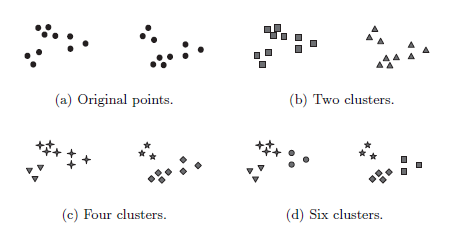
\includegraphics[width= 8cm, height= 6cm]{doc/DokumenSkripsi/Gambar/gambar21.PNG}
    \caption{Perbedaan cara \textit{clustering}}
    \label{fig:perbedaan cara clustering}
\end{figure}

\subsection{Jenis-Jenis \textit{Clustering}}
\label{subsec:jenis clustering}

Seluruh kumpulan cluster biasanya disebut sebagai \textit{clustering}, berikut merupakan jenis-jenis dari \textit{clustering} \cite{buku:data:mining} :

\begin{enumerate}
    \item \textit{Hierarchical versus Partitional} \\
        Pengelompokkan partional adalah sebuah pembagian set objek data kedalam subset (\textit{cluster}) yang tidak tumpang tindih sehingga setiap objek data berada dalam satu subset. Pada gambar \ref{fig:perbedaan cara clustering} adalah contoh pengelompokkan parsial.
        
        Pengelompokkan hierarkis adalah kumpulan \textit{cluster} bertingkat uang diorganisasikan sebagai \textit{tree}. Setiap node (\textit{cluster}) di \textit{tree} (kecuali untuk \textit{leaf node}) adalah \textit{subcluster} dan \textit{root} adalah \textit{cluster} yang berisikan semua objek data.
    
    \item \textit{Exclusive versus Overlapping versus Fuzzy} \\
        Gambar \ref{fig:perbedaan cara clustering} merupakan pengelompokkan yang eksklusif, karena setiap objek berada didalam satu \textit{cluster}. Dalam situasi tertentu suatu objek dapat ditempatkan di lebih dari satu \textit{cluster}, untuk kasus seperti ini dapat di tangani oleh non-eksklusif atau \textit{overlapping}. \textit{Overlapping} digunakan untuk menggambarkan fakta bahwa suatu objek dapat secara bersamaan berada di lebih dari satu kelompok. Misalnya, seseorang di universitas dapat terdaftar sebagai mahasiswa dan karyawan.
        
        Dalam pengelompokkan fuzzy, setiap objek berada di setiap kelompok dengan bobot keanggotaan antara 0 (tidak termasuk dalam kelompok) dan 1 (termasuk dalam kelompok). Secara matematis himpunan fuzzy adalah himpunan di mana objek berada didalam setiap kelompok dengan bobot kenanggotaan 0 sampai 1. Karena bobot keanggotaan untuk objek berjumlah 1, pengelompokkan fuzzy tidak membahas situasi \textit{multiclass} yang sebenarnya, seperti kasus seorang mahasiswa yang segaligus karyawan pada sebuah universitas. Dalam praktiknya, pengelompokkan fuzzy sering dikonversi menjadi pengelompokkan eksklusif dengan menetepkan setiap objek kedalam kelompok dengan bobot keanggotaan tertinggi.
        
    \item \textit{Complete versus Partial}
        Pengelompokkan lengkap menetapkan setiap objek ke sebuah kelompok, sedangakan pengelompokan parsial tidak. Motivasi dari pengelompokkan parsial adalah bahwa beberapa objek dalam kumpulan data mungkin bukan milik kelompok yang terdefinisi dengan baik. Banyak objek dalam kumpulan data dinyatakan sebagai \textit{noise}, \textit{outlier}, atau \textit{“uninteresting background”}.
    
\end{enumerate}


\subsection{Jenis-Jenis \textit{Cluster}}
\label{subsec:jeni cluster}
\textit{Clustering} bertujuan untuk menemukan kelompok objek yang berguna, dimana kegunaan didefinisikan dengan tujuan analisis data. Terdapat beberapa konsep berbeda tentang \textit{cluster} yang dapat digunakan dalam praktik. Gambar \ref{fig:jenis cluster} merupakan contoh secara visual perbedaan diantara tipe-tipe \textit{cluster}, dengan menggunakan ruang dua dimensi. Berikut merupakan jenis-jenis \textit{cluster} \cite{buku:data:mining} :

\begin{enumerate}
    \item \textit{Well-Separated} \\
        \textit{Cluster} adalah kumpulan objek dimana setiap objek dianggap dekat atau mirip dengan obejk di \textit{cluster} yang sama. \textit{Threshold} biasanya digunakan untuk menentukan bahawa semua objek dalam \textit{cluster} cukup mirip atau dekat satu sama lain. Gambar \ref{fig:jenis cluster} (a) memberikan contoh kelompok yang terpisah dengan baik yang terdiri dari dua kelompok dalam ruang dua dimensi. \textit{Cluster} yang dipisahkan dengan baik tidak harus berbentuk bola, tetapi dapat dalam bentuk lain.
        
    \item \textit{Prototype-Based} \\
        \textit{Cluster} kumpulan objek dimana setiap objek lebih dekat atau mirip dengan prototipe yang mendefinisiakan \textit{cluster} dari pada prototipe \textit{cluster} lain. Untuk data dengan atribut kontinu, prototipe \textit{cluster} sering kali merupakan \textit{centroid}. \textit{Centroid} adalah rata-rata dari semua titik atau titik tengah dari \textit{cluster}. Ketika \textit{centroid} tidak dapat digunakan, seperti ketika data memiliki atribut kategorikal, prototipe sering kali disebut \textit{medoid}. \textit{Medoid} adalah titik representatif dari sebuah \textit{cluster}. Untuk beberapa jenis data, prototipe dianggap sebagai titik paling central, kelompok\textit{prototype-based} dianggap sebagai kelompok \textit{center-based}. \textit{Cluster} seperti ini cenderung bulat seperti pada gambar \ref{fig:jenis cluster} (b).
            
    \item \textit{Graph-Based}\\
        Jika data direpresentasikan sebagai garik, dimana node adalah objek dan \textit{link} mewakili hubungan antara objek, maka sebuah \textit{cluster} dapat didefinisikan sebagai komponen yang terhubung, seperti sekelompok objek yang terhubung satu sama lain, tetapi tidak memiliki hubungan dengan objek diluar kelompok objek saat ini. Contoh penting dari \textit{cluster} berbasis grafik adalah \textit{cluster} berbasis kontiguitas, dimana dua objek terhubung hanya jika mereka berada dalam jarak yang ditentukan satu sama lain. Gambar \ref{fig:jenis cluster} (c) menunjukkan contoh dari cluster berbasis kontiguitas untuk ruang dua dimensi. Terdapat masalah ketia terdapat \textit{noise}, seperti pada gambar \ref{fig:jenis cluster} (c) jembatan dapat menghubungkan dua \textit{cluster} yang berbeda.
        
    \item \textit{Density-Based} \\
        \textit{Cluster} adalah daerah padat dari objek yang dikelilingi oleh daerah yang kepadatannya rendah. \ref{fig:jenis cluster} (d) menunjukkan beberapa \textit{cluster} berbasis kepadatan untuk data yang dibuat dengan menambahkan \textit{noise} ke data pada gambar \ref{fig:jenis cluster} (c). Kedua \textit{cluster} tidak terhubung dengan jembatan, karena jembatan diantara \textit{cluster} menjadi \textit{noise}. \textit{Cluster} berbasis kepadatan biasa digunakan ketika data tidak teratur dan terdapat \textit{noise} dan \textit{outlier}. 
        
    \item \textit{Shared-Property (Conceptual Clusters)}
        Secara lebih umum, \textit{cluster} adalah sebagai satu kumpulan objek yang berbagi beberapa properti. Definisi ini mencakup semua definisi \textit{cluster} sebelumnya, seperti objek dalam \textit{cluster} berbasis pusat berbagi properti yang sama dengan semua yang paling dekat dengan \textit{centroid} atau \textit{medoid} yang sama. Namun pendekatan ini juga mencakup ide baru. Sebagai contoh pada gambar \ref{fig:jenis cluster} (e), daerah dengan bentuk segitiga berdekatan dengan daerah berbentuk persegi panjang dan terdapat dua lingkaran yang saling beririsan. Dalam kedua kasus tersebut, algoritma pengelompokan akan membutuhkan konsek \textit{cluster} yang sangat spesifik untuk berhasil mendeteksi \textit{cluster} seperti pada gambar \ref{fig:jenis cluster} (e). Proses penemuan \textit{cluster} tersebut disebut \textit{conceptual clustering}.
        
    \item \textit{Road Map}
        Berikut merupakan tiga teknik sederhana didalam \textit{road map} :
        
        \begin{enumerate}
            \item K-Means\\
                K-Means adalah teknik pengelompokan partisionalmberbasis prototipe yang mencoba untuk menemukan jumlah \textit{cluster} (k) yang ditentukan pengguna, yang mewakili centroid.
            
            \item \textit{Agglomerative Hierarchical Clustering}\\
                Pendekatan pengelompokan ini mengacu pada kumpulan teknik pengelompokan yang terkait erat yang menghasilkan pengelompokan hierarkis dengan memulai dengan setiap objek sebagai satu \textit{cluster} dan kemudia berulang kali menggabungkan dua \textit{cluster} terdekat menjadi satu, semua \textit{cluster}  yang tersisa tetap ada.
            
            \item DBSCAN \\
                DBSCAN adalah algoritma pengelompokan berbasis kepadatan yang menghasilkan pengelompokan parsial, dimana jumlah \textit{cluster} secara otomatis ditentukan algoritma. 
            
        \end{enumerate}
    
\end{enumerate}


\begin{figure}[H]
    \centering
    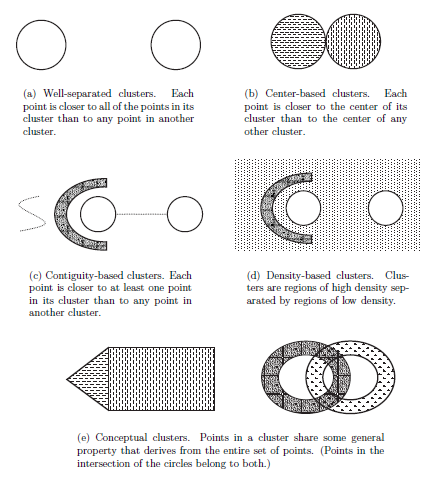
\includegraphics[width = 10cm, height = 12cm]{doc/DokumenSkripsi/Gambar/gambar22.PNG}
    \caption{Jenis-Jenis \textit{Cluster}}
    \label{fig:jenis cluster}
\end{figure}



\subsection{K-Means}
\label{subsec:dasar teori K-Means}
K-Means \cite{buku:data:mining} mendefinisikan prototipe dalam hal centroid, yang biasanya merupakan rata-rata dari sekelompok data dan biasanya diaplikasikan pada objek dalam ruang n dimensi.

\begin{enumerate}
    \item Dasar Algoritma K-Means \\
        Berikut merupakan tahapan-tahapan pada dasar algoritma K-Means :
        
        \begin{enumerate}
            \item Memilih K \textit{centroid} awal, dimana K adalah parameter yang ditentukan oleh pengguna. K adalah jumlah \textit{cluster} yang akan dibentuk.
            
            \item Menempatkan semua data ke \textit{centroid} terdekat.
            
            \item Menghitung \textit{centroid} baru berdasarkan data yang berada didalam \textit{cluster}.
            
            \item Mengulang tahap b-c sampai tidak ada data yang mengubah \textit{cluster}, sehingga \textit{centroid} tetap sama.
        \end{enumerate}
\end{enumerate}

Gambar \ref{fig:ilustrasi K-Means} merupakan ilustrasi dari operasi K-Means yang menunjukan bagaimana pembentukan tiga \textit{cluster} dalam empat kali pengulangan. Setiap sub-gambar akan menunjukkan \textit{centroid} awal dan penempatan data ke \textit{centroid}. \textit{Centroid} ditandai menggunakan simbol "+", sedangkan data yang bukan \textit{centroid} menggunakan simbol segitiga. 

Langkah pertama seperti pada gambar \ref{fig:ilustrasi K-Means} (a), memilih \textit{centroid} awal, menempatkan data ke \textit{centroid} terdekat, dan menghitung centroid baru. Pada langkah kedua, menempatkan data ke \textit{centroid} baru, dan menghitung \textit{centroid} baru. Pada langkah 2, 3, dan 4 ditunjukkan pada gambar \ref{fig:ilustrasi K-Means} (b), (c), dan (d). Algoritma K-Means berakhir pada gambar \ref{fig:ilustrasi K-Means} (d), karena tidak ada lagi perubahan yang terjadi.

\begin{figure}[H]
    \centering
    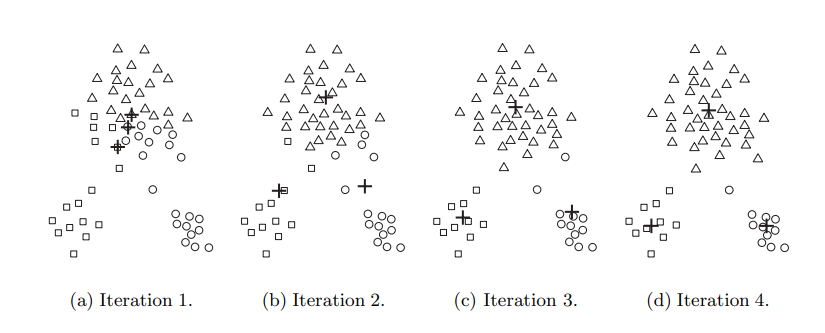
\includegraphics[width= 10cm, height=6cm]{doc/DokumenSkripsi/Gambar/gambar23.PNG}
    \caption{Penggunaan K-Means untuk Menemukan Tiga \textit{Cluster}}
    \label{fig:ilustrasi K-Means}
\end{figure}

Pada bagian ini akan dijelaskan tahap-tahap pada dasar algoritma K-Means lebih dalam.

\begin{enumerate}
    \item Memilih K \textit{centroid} awal \\
        Pemilihan \textit{centroid} awal dilakukan secara acak, setiap kali algoritma K-Means dijalankan, akan menghasilkan \textit{cluster} yang berbeda-beda.
        
    \item Menempatkan semua data ke \textit{centroid} terdekat\\
        Untuk menempatkan data ke \textit{centroid} terdekat dibutuhkan ukuran kedekatan. \textit{Euclidean distance} sering digunakan untuk data dalam ruang \textit{Euclidean}, sedangkan \textit{cosine similariy} lebih sesuai untuk dokumen.
            
    \item Menghitung \textit{centroid} baru\\
        Pehitungan \textit{centroid} baru dilakukkan dengan cara menghitung rata-rata berdasarkan data yang terdapat pada \textit{cluster}.
\end{enumerate}

Salah satu masalah dalam dasar algoritma K-Means adalah \textit{cluster} kosong yang terjadi karena tidak ada data yang dotempatkan pada \textit{cluster} tersebut. Jika ini terjadi, maka diperlukan cara untuk memilih centroid pengganti. Salah satu cara yang dapat dilakukan adalah memilih data yang jauh dari \textit{centroid} saat ini.


\section{\textit{Library} PHP-ML}
\label{sec:library php-ml}
%Penjelasan php ml
PHP-ML adalah sebuah \textit{library} yang khusus dibuat untuk \textit{Machine Learning} dengan menggunakan bahasa pemrograman PHP. Terdapat lebih dari 20 algoritma yang bisa digunakan. \textit{Library} ini bersifat \textit{open source} yang berlisensi MIT. Versi PHP minimal untuk menggunakan \textit{library} ini adalah PHP 7.1, pengingstallan dapat menggunakan Composer.

% https://php-ml.readthedocs.io/en/latest/machine-learning/datasets/array-dataset/
\subsection{Array Dataset} % perlu di italic atau engga
\textit{Array Dataset} adalah bagian dari fitur \textit{Dataset} yang disediakan oleh PHP-ML. \textit{Array Dataset} adalah kelas yang berfungsi untuk menyimoan data sebagai tipe array dalam PHP. Menerapkan \textit{interface} Dataset yang banyak digunakan di kelas lain. Kelas ini memiliki dua parameter yaitu : \textit{samples} dan \textit{labels}. \textit{Samples} adalah array yang berisikan sample. \textit{Labels} adalah array yang berisikan \textit{label} setiap \textit{sample}.

% https://php-ml.readthedocs.io/en/latest/machine-learning/cross-validation/random-split/
\subsection{Random Split}
\textit{Random Split} adalah bagian dari fitur \textit{Cross Validation} yang disediakan oleh PHP-ML. Kelas \textit{Random Split} adalah salah satu metode paling sederhana dari \textit{Cross Validation}. \textit{Samples} dibagi menjadi dua kelompok yaitu : \textit{train group} dan \textit{test group}. Kelas ini memiliki tiga parameter yaitu : \textit{dataset}, \textit{testSize}, dan \textit{seed}. \textit{Dataset} adalah objek yang mengimplementasikan \textit{interface} Dataset. \textit{TestSize} adalah bilangan \textit{float} yang menyatakan seberapa banyak anggota pada \textit{test group} dengan nilai dasar 0.3 jika parameter tidak diisi. \textit{Seed} untuk \textit{random generator}.

\section{Universitas Katolik Parahyangan}
\label{sec:unpar}

%\subsection{Universitas Katolik Parahyangan}
Perguruan tinggi adalah satuan pendidikan yang menyelenggarakan pendidikan tinggi yang dapat berbentuk akademi, politeknik, sekolah tinggi, institut. atau universitas. Pendidikan tinggi adalah kelanjutan pendidikan menengah yang diselenggarakan untuk menyiapkan peserta didik menjadi anggota masyarakat yang memiliki kemampuan akademik dan/atau profesional yang dapat menerapkan, mengembangkan dan/atau menciptakan ilmu pengetahuan. teknologi dan/atau kesenian. %SK MENDIKNAS 232

Universitas Katolik Parahyangan adalah sebuah univessitas atau Perguruan tinggi katolik pertama yang didirikan pada 17 Januari 1955. Saat ini terletak di Jalan Ciumbuleuit No.94, Bandung, Jawa Barat, Indonesia. Terdapat tujuh fakultas dengan total program studi yaitu tujuh belas dengan enam belas program studi sarjana dan satu program studi D3. %unpar.ac.id

Terdapat beberapa jalur penerimaan mahasiswa baru yang dilakukan oleh Universitas Katolik Parahyangan. Jalur penerimaan diselenggarakan secara mandiri, berikut jalur penerimaan yang disediakan Universitas Katolik Parahyangan :

\begin{enumerate}
	\item Penelusuran Minat dan Kemampuan (PMKD) atau jalur prestasi\\
		PMDK adalah satu jalur penerimaan mahasiswa baru yang dilaksakan dengan seleksi berdasarkan pada nilai raport SMA di kelas X (Sepuluh) dan XI (Sebelas), tanpa ujian tertulis. Tujuan dari PMDK untuk menjaring siswa-siswa yang berprestasi. PMDK dilakukan hanya satu kali dalam satu tahun penerimaan.
		
	\item Ujian Saringan Masuk (USM)\\
		USM adalah satu jalur penerimaan mahasiswa baru yang dilaksanakan dengan mengerjakan soal yang disediakan oleh Universitas Katolik Parahyangan. Terdapat dua tempat pelaksanaan untuk USM, pertama dilaksakan di Universitas Katolik Parahyangan dan kedua dilaksakan di sekolah-sekolah (\textit{on-site test}.Tujuan dari USM untuk menjaring mahasiswa baru yang memiliki kemampuan akademik untuk mengikuti dan menyelesaikan pendidikan di Universitas Katolik Parahyangan sesuai dengan batas waktu (masa studi) yang ditetapkan.
	
\end{enumerate}

\subsection{Program Studi}
\label{sec:program studi} 
%Diisi dengan penjelasan program studi dan syarat-syaratnya
Program studi adalah kesatuan rencana belajar sebagai pedoman penyelenggaraan pendidikan akademik dan/atau profesional yang diselenggarakan atas dasar suatu kurikulum serta ditujukan agar mahasiswa dapat menguasai pengetahuan, keterampilan, dan sikap sesuai dengan sasaran kurikulum. Kurikulum pendidikan tinggi adalah seperangkat rencana dan pengaturan mengenai isi maupun bahan kajian dan pelajaran serta cara penyampaian dan penilaiannya yang digunakan sebagai pedoman penyelenggaraan kegiatan belajar - mengajar di perguruan tinggi.  %SK MENDIKNAS 232

Terdapat tujuh fakultas yang ada di Universitas Katolik Parahyangan, yaitu :
	\begin{enumerate}
		\item Fakultas Ekonomi 
		\item Fakultas Hukum
		\item Fakultas Ilmu Sosial dan Ilmu Politik
		\item Fakultas Teknik
		\item Fakultas Falsafah dan Peradaban
		\item Fakultas Teknologi Industri
		\item Fakultas Teknologi Informasi dan Sains
	\end{enumerate}\leavevmode
	
\subsubsection{Fakultas Ekonomi}
Terdapat empat program studi pada fakultas Ekonomi, yaitu : Ekonomi Pembangunan, Manajemen, Akuntansi, Manajemen Perusahaan. Manajemen Perusahaan merupakan program studi D3 yang ada di Universitas Katolik Parahyangan. Berikut merupakan penjelasan program studi yang ada pada Fakultas Ekonomi :
	
	\begin{enumerate}
		\item Ekonomi Pembangunan\\
			 Mempelajari persoalan pembangunan ekonomi yang sudah, sedang, dan akan
terjadi di negara berkembang. Menganalisis isu perekonomian untuk mencari dan menemukan solusi dari berbagai persoalan ekonomi secara kritis, kreatif, dan inovatif. Program studi Ekonomi Pembangunan mempersiapkan mahasiswanya untuk menjadi perencana bidang pembangunan ekonomi. Ekonomi Pembangunan adalah cabang ilmu ekonomi. Mempelajari pembangunan industri, perbankan, keuangan, dan bisnis. Berkutat dengan analisis berbagai isu perekonomian untuk mendapatkan solusi dari persoalan ekonomi.

			Terdapat tiga peminatan pada program studi Ekonomi Pembangunan, yaitu :
			\begin{itemize}
				\item Ekomoni Industri dan Perdagangan
				\item Ekonomi Kawasan dan Lingkungan
				\item Ekonomi Moneter dan Keuangan
			\end{itemize}\leavevmode

		\item Manajemen\\
			Mempelajari bagaimana mengelola suatu perusahaan atau organisasi. Fokus pada kegiatan mengelola, merencanakan, dan mengatur semua proses dalam perusahaan untuk mencapai tujuan.
			
			Terdapat satu peminatan pada program studi Manajemen, yaitu :
			\begin{itemize}
				\item Manajemen
			\end{itemize}\leavevmode

		\item Akuntansi\\
			Mempelajari mengenai keuangan dan ilmu ekonomi, Mahasiswa pada program studi Akuntansi akan memiliki pengetahuan dan penguasaan materi tentang keuangan dan ilmu ekonomi. Mampu mengelola keuangan bisnis.
			
			Terdapat satu peminatan pada program studi Akuntansi, yaitu :
			\begin{itemize}
				\item Akuntansi
			\end{itemize}\leavevmode
		
		%\item Manajemen Perusahaan\\
			%Terdapat satu peminatan pada program studi Manajemen Perusahaan, yaitu :
			%\begin{itemize}
				%\item Manajemen Perusahaan
			%\end{itemize}\leavevmode
			
	\end{enumerate}\leavevmode

\subsubsection{Fakultas Hukum}
Terdapat satu program studi pada Fakultas Hukum, yaitu : Ilmu Hukum.

	%program studi
	\begin{enumerate}
		\item Ilmu Hukum\\
			Mempelajari tentang hukum baik praktek maupun teori. Hukum mengatur bagaimana manusia bertindak dan bertingkah laku agar tidak merugikan orang lain. Mendalami konsep, teori, dan beberapa kasus hukum yang terjadi.
			
			Terdapat satu peminatan pada program studi Ilmu Hukum, yaitu :
			
			\begin{itemize}
				\item Ilmu Hukum
			\end{itemize}\leavevmode
			
	\end{enumerate}\leavevmode

\subsubsection{Fakultas Ilmu Sosial dan Ilmu Politik}
Terdapat tiga program studi pada Fakultas Ilmu Sosial dan Ilmu Politik, yaitu : Ilmu Administrasi Publik, Ilmu Administrasi Bisni, dan Ilmu Hubungan Internasional.
	%program studi
	\begin{enumerate}
		\item Ilmu Administrasi Publik\\
			Mempelajari seluk beluk pemerintahan, masyarakat, dan kebijakan publik, sistem pemerintahan, pembuatan kebijakan hingga pengimplementasian dan evaluasi, pelayanan masyarakat, dan segala sesuatu yang berkaitan dengan birokrasi.

			Terdapat satu peminatan pada program studi Ilmu Administrasi Publik, yaitu :
			
			\begin{itemize}
				\item Ilmu Administrasi Publik
			\end{itemize}\leavevmode
			
		\item Ilmu Administrasi Bisnis\\
			Mempelajari mengenai kegiatan operasional bisnis dan perusahaan, yaitu : pemasaran (marketing), pengelolaan keuangan, pengelolaan personalia (SDM), hingga kegiatan produksi. Mempelajari untuk membuat produk sendiri, bukan membuat, menjual, dan mendapatkan keuntungan, tetapi menciptakan value pada produk yang dipasarkan. Mempelajari urusan klarikal kantor, mengelola sarana dan prasarana kantor, memproses data secara akurat, dan mengelola informasi yang berhubungan dengan pekerjaan kantor. Program studi ini cocok dengan orang yang memiliki ketertarikan dalam bidang pengurusan dokumen.
			
			Terdapat dua peminatan pada program studi Ilmu Administrasi Bisnis, yaitu :
			
			\begin{itemize}
				\item \textit{General Business}
				\item \textit{Digital Business}
			\end{itemize}\leavevmode
						
		\item Ilmu Hubungan Internasional\\
			Mempelajari mengenai interaksi, relasi, dan komunikasi yang terjadi secara internasional. Tidak hanya mempelajari hubungan diplomasi satu negara dengan negara lain, tapi juga konflik, kesejahteraan, ekonomi, dan perdamaian dunia. Beberapa kajian diplomasi dan negosiasi, politik luar negeri, perdagangan luar negeri, politik internasional, ekonomi internasional, hukum internasional, globalisasi, dll. Diasah mengenai isu-isu global, tokoh-tokoh, dan organisasi internasional yang berpengaruh, dan kerjasama internasional.
			
			Terdapat satu peminatan pada program studi Ilmu Administrasi Bisnis, yaitu :
			
			\begin{itemize}
				\item Ilmu Hubungan Internasional
			\end{itemize}\leavevmode

	\end{enumerate}\leavevmode
	
\subsubsection{Fakultas Teknik}
Terdapat dua program studi pada Fakultas Teknik, yaitu : Teknik Sipil dan Arsitektur.
	%program studi
	\begin{enumerate}
		\item Teknik Sipil\\
			 Mempelajari proses merancang, membangun, dan merenovasi gedung serta infrastruktur lain, seperti jalan, jembatan, bendungan, dan infrastruktur lainnya. Memahami unsur-unsur bangunan seperti beton, baja, aspal, dan lain-lain. Mempelajari perancangan struktur bangunan yang kuat, layak, dan efisien.
			
			Terdapat satu peminatan pada program studi Teknik Sipil, yaitu :
			
			\begin{itemize}
				\item Teknik Sipil
			\end{itemize}\leavevmode
			
		\item Arsitektur\\
			Mempelajari desain dan rancangan konstruksi bangunan. Lebih menuangkan ide, konsep, dan desain di atas kertas, sedangkan realisasi akan dikerjakan oleh teknik sipil. Harus mempelajari kekuatan bangunan (firmitasi), estetika atau keindahan bangunan (venustas), dan fungsi bangunan (utilitas).
			
			Terdapat satu peminatan pada program studi Arsitektur, yaitu :
			
			\begin{itemize}
				\item Arsitektur
			\end{itemize}\leavevmode

	\end{enumerate}\leavevmode
	
\subsubsection{Fakultas Falsafah dan Peradaban}
Terdapat satu program studi pada Fakultas Falsafah dan Peradaban, yaitu : Ilmu Filsafat.
	
	%program studi
	\begin{enumerate}
		\item Ilmu Filsafat\\
			 Filsafat sebagai induk semua ilmu, filsafat lebih mempelajari tentang permasalahan mendasar manusia dan hubungannya dengan realita. Bersifat abstrak dan memerlukan pemahaman yang mendasar. Kajian utamanya yaitu tujuan hidup, esensi manusia, moralitas, dan hati nurani. Mempelajari pemikiran para filsuf. Membantu berpikir secara terstruktur dan mampu memproses informasi secara jernih.
			
			Terdapat dua peminatan pada program studi Ilmu Filsafat, yaitu :
			
			\begin{itemize}
				\item Filsafat Keilahian
				\item Filsafat Budaya
			\end{itemize}\leavevmode
			
	\end{enumerate}\leavevmode
	
\subsubsection{Fakultas Teknologi Industri}
Terdapat tiga program studi pada Fakultas Teknologi Industri, yaitu : Teknik Industri, Teknik Kimia, dan Teknik Elektro.
	%program studi
	\begin{enumerate}
		\item Teknik Industri\\
			Mempelajari proses industri baik dari sisi manajemen ataupun teknik. Turunan dari teknik mesin. Mempelajari disiplin ilmu lain seperti matematika, fisika, fisiologi, dan manajemen saintifik. Teknik Industri berfokus pada perancangan, peningkatan, dan pemasangan sistem terintegrasi yang membutuhkan manusia, material, peralatan, dan energi. Memiliki tiga bidang dan satu sistem manufaktur (mempelajari peningkatan kualitas, produktivitas, dan efisiensi sistem produk), dua manajemen industri (mempelajari manajemen keuangan, operasional, manajemen inovasi, perencanaan dan pengendalian produksi, dan ekonomi teknik), dan tiga sistem industri dan tekno ekonomi, seperti logistik, statistik, penelitian operasional, dan sistem basis data.
			
			Terdapat satu peminatan pada program studi Teknik Industri, yaitu :
			
			\begin{itemize}
				\item Teknik Industri
			\end{itemize}\leavevmode
			
		\item Teknik Kimia\\
			Cabang ilmu teknik yang mempelajari bagaimana proses dan cara mengubah bahan baku/mentah dan bahan kimia menjadi sebuah produk yang lebih bernilai secara komersial maupun perubahan sifat fisik dan kimia bahan mentah. Dididik untuk merencanakan dan merancang alat-alat proses, mengoperasikan, mengendalikan dan memelihara pabrik/industri, mengkontruksi pendirian suatu pabrik, mengadakan penelitian dan pengembangan proses, serta merencanakan serta mengelola penjualan dan pelayanan.
			
			Terdapat satu peminatan pada program studi Teknik Kimia, yaitu :
			
			\begin{itemize}
				\item Teknik Kimia
			\end{itemize}\leavevmode

		\item Teknik Elektro\\
			Mempelajari sifat-sifat elektron yang kita kenal sebagai listrik, mempelajari aplikasi dan pemanfaatan listrik dalam kehidupan sehari-hari, serta teknologi yang terkait. Cakupannya meliputi pembangkit tenaga listrik, sistem jaringan distribusi, pemanfaatan oleh pengguna akhir.
			
			Terdapat satu peminatan pada program studi Teknik Elektro, yaitu :
			
			\begin{itemize}
				\item Mekatronika
			\end{itemize}\leavevmode

	\end{enumerate}
	
\subsubsection{Fakultas Teknologi Informasi dan Sains}
Terdapat tiga program studi pada Fakultas Teknologi Informasi dan Sains, yaitu : Matematika, Fisika, dan Teknik Informatika.
	
	%program studi
	\begin{enumerate}
		\item Matematika\\
			Mempelajari matematika murni seperti aljabar, geometri, dan analisis matematika; statistika; komputasi; aktuaria; dan riset operasi.

			Terdapat dua peminatan pada program studi Matematika, yaitu :
			
			\begin{itemize}
				\item Aktuaria
				\item Matematika Terapan
			\end{itemize}\leavevmode
			
		\item Fisika\\
			 Mempelajari gejala alam yang tidak hidup atau materi dalam lingkup ruang dan waktu, mempelajari perilaku dan sifat materi dalam bidang yang sangat beragam (partikel submikroskopis - perilaku materi alam semesta sebagai satu kesatuan kosmos). Ilmu fisika sangat mendukung perkembangan teknologi, yaitu industri, komunikasi, kerekayasaan, kimia, dan kedokteran.
			 
			 Terdapat satu peminatan pada program studi Fisika, yaitu :
			
			\begin{itemize}
				\item Fisika
			\end{itemize}\leavevmode

		\item Teknik Informatika\\
			Mempelajari dan menerapkan prinsip-prinsip ilmu komputer dan analisa matematis untuk desain, pengembangan, pengujian, evaluasi perangkat lunak, sistem operasi, dan kerja komputer. Menghasilkan ide kreatif, merealisasikan ide, mendiferensiasikan berbagai macam fungsi, dan menciptakan struktur instruksi yang sangat detail dalam bahasa pemrograman untuk mengajarkan komputer apa yang harus dilakukan.
			
			Terdapat dua peminatan pada program studi Teknik Informatika, yaitu :
			
			\begin{itemize}
				\item \textit{Data Science}
				\item \textit{Computer Science}
			\end{itemize}\leavevmode
			
	\end{enumerate}\leavevmode
	
\subsection{Syarat Masuk Program Studi}
Berikut merupakan syarat untuk program studi yang ada di Universitas Katolik Parahyangan :
\begin{longtable}[H]{|p{3cm}|p{2cm}|p{3cm}|p{3cm}|p{3cm}|} %atau h saja untuk "kira kira di sini"
	%\centering 

	%\begin{tabular}{|p{3cm}|p{2cm}|p{3cm}|p{3cm}|p{3cm}|}
		\hline
		Program Studi & Syarat Jurusan & USM  & PMDK & Syarat Khusus \\

		\hline
		\multirow{3}{10em}{Ekonomi Pembangunan} & IPA & Matematika & Matematika & \\
		& IPS & Bahasa Inggris & Bahasa Indonesia & \\
		& & & Bahasa Inggris & \\
		
		\hline
		\multirow{2}{10em}{Manajemen} & IPA & Matematika & Matematika & \\
		& IPS & Bahasa Inggris & Bahasa Inggris & \\
		
		\hline
		\multirow{2}{10em}{Akuntansi} & IPA & Matematika & Matematika & \\
		& IPS & Bahasa Inggris & Bahasa Inggris & \\
		
		%\hline
		%\multirow{4}{10em}{Manajemen Perusahaan} & IPA & Esai & Matematika & \\
		%& IPS & & & \\
		%& Bahasa & & & \\
		%& SMK & & & \\
		
		\hline
		\multirow{3}{10em}{Ilmu Hukum} & IPA & Matematika & Matematika & \\
		& IPS & Bahasa Inggris & Bahasa Inggris & \\
		& Bahasa & & Pendidikan Kewarganegaraan & \\
		
		\hline
		\multirow{4}{10em}{Ilmu Administrasi Publik} & IPA & Matematika & Matematika & \\
		& IPS & Bahasa Inggris & Bahasa Inggris & \\
		& Bahasa & & & \\
		& SMK & & & \\
		
		\hline
		\multirow{4}{10em}{Ilmu Administrasi Bisnis} & IPA & Matematika & Matematika & \\
		& IPS & Bahasa Inggris & Bahasa Inggris & \\
		& Bahasa & & & \\
		& SMK & & & \\
		
		\hline
		\multirow{3}{10em}{Ilmu Hubungan Internasional} & IPA & Matematika & Matematika & \\
		& IPS & Bahasa Inggris & Bahasa Inggris & \\
		& Bahasa & & Uraian Bahasa Inggris & \\
		
		\hline
		\multirow{3}{10em}{Teknik Sipil} & IPA & Matematika & Matematika & \\
		& & Bahasa Inggris & Bahasa Inggris & \\
		& & Fisika & Fisika & \\
		
		\hline
		\multirow{3}{10em}{Arsitektur} & IPA & Matematika & Matematika & \\
		& & Bahasa Inggris & Bahasa Inggris & \\
		& & Gambar & Gambar & \\
		
		\hline
		\multirow{4}{10em}{Ilmu Filsafat} & IPA & Matematika & Bahasa Inggris & \\
		& IPS & Bahasa Inggris & Bahasa Indonesia & \\
		& Bahasa & Wawancara & & \\
		& SMK & & & \\
		
		\hline
		\multirow{2}{10em}{Teknik Industri} & IPA & Matematika & Bahasa Inggris & \\
		& & Matematika & Bahasa Inggris & \\
		
		\hline
		\multirow{4}{10em}{Teknik Kimia} & IPA & Matematika & Matematika & Tidak buta warna\\
		& & Bahasa Inggris & Bahasa Inggris & \\
		& & Fisika & Fisika & \\
		& & & Kimia & \\
		
		\hline
		\multirow{3}{10em}{Teknik Elektro} & IPA & Matematika & Matematika & Tidak buta warna \\
		& & Bahasa Inggris & Bahasa Inggris & \\
		& & Fisika & Fisika & \\
		
		\hline
		\multirow{2}{10em}{Matematika} & IPA & Matematika & Matematika & \\
		& & Bahasa Inggris & Bahasa Inggris & \\
		& & & & \\
		
		\hline
		\multirow{3}{10em}{Fisika} & IPA & Matematika & Matematika & \\
		& & Bahasa Inggris & Bahasa Inggris & \\
		& & Fisika & & \\
		
		\hline
		\multirow{2}{10em}{Teknik Informatika} & IPA & Matematika & Matematika & \\
		& & Bahasa Inggris & Bahasa Inggris & \\
		
		\hline
	%\end{tabular} 
	\caption{Tabel syarat program studi}
	\label{tab:tabel syarat program studi}
\end{longtable}

\subsection{Karakteristik Program Studi}
Berikut merupakan kriteria untuk calon mahasiswa sesuai dengan program studi :



\begin{longtable}[H]{| p{6cm} | p{8cm} |} %atau h saja untuk "kira kira di sini"
	%\centering 
	%\begin{tabular}
		\hline
		Program Studi & Karakteristik \\

		\hline
		\multirow{5}{10em}{Ekonomi Pebangunan} & Tertarik dengan Ilmu Ekonomi \\
		& Tertarik dengan perhitungan \\
		& Berpikir kritis \\
		& Senang menganalisis\\
		& Mampu memecahkan masalah\\
		
		\hline
		\multirow{3}{10em}{Manajemen} & Keterampilan komunikasi \\
		& Senang menganalisis\\
		& Senang memecahkan masalah\\
		
		\hline
		\multirow{3}{10em}{Akuntansi} & Tertarik dengan akuntansi \\
		& Memiliki kemampuan berhitung yang kuat dan teliti \\
		& Senang menganalisis\\
		
		\hline
		%\multirow{3}{10em}{Manajemen Perusahaan} &  \\
		%& \\
		%& \\
		
		\hline
		\multirow{4}{10em}{Ilmu Hukum} & Tertarik dengan hukum \\
		& Teliti dan berpikir kritis \\
		& Keterampilan komunikasi \\
		& Mampuan menganalisis\\
		
		\hline
		\multirow{3}{10em}{Ilmu Administrasi Publik} & Terstruktur \\
		& Senang menganalisis\\
		& Senang memecahkan masalah\\
		
		\hline
		\multirow{4}{10em}{Ilmu Administrasi Bisnis} & Memiliki minat yang tinggi untuk usaha \\
		& Kemampuan komunikasi\\
		& Kemampuan berhitung\\
		& Terstruktur\\
		
		\hline
		\multirow{4}{10em}{Ilmu Hubungan Internasional} & Tertarik dengan interaksi internasional \\
		& Kemampuan berbahasa Inggris \\
		& Berwawasan luas \\
		& Kemampuan komunikasi\\
		
		\hline
		\multirow{2}{10em}{Teknik Sipil} & Senang berhitung \\
		& Terstruktur \\
		
		\hline
		\multirow{4}{10em}{Arsitektur} & Tertarik dengan desain dan rancangan bangunan \\
		& Tertarik dengan menggambar dan seni\\
		& Tertarik dengan humaniora, sains, dan teknologi \\
		
		\hline
		\multirow{4}{10em}{Ilmu Filsafat} & Tipe pemikir \\
		& Berwawasan luas \\
		& Berpikir Rasional \\
		& Berpikir kritis \\
		
		\hline
		\multirow{2}{10em}{Teknik Industri} &  Senang berhitung \\
		& Terstruktur \\
		
		\hline
		\multirow{4}{10em}{Teknik Kimia} & Tertarik dengan Kimia \\
		& Senang berhitung \\
		& Terstruktur \\
		& Tidak buta warna\\
		
		\hline
		\multirow{4}{10em}{Teknik Elektro} & Tidak buta warna \\
		& Senang berhitung \\
		& Terstruktur \\
		& Teliti \\

		\hline
		\multirow{4}{10em}{Matematika} & Tertarik dengan Matematika \\
		& Senang memecahkan masalah \\
		& Terstruktur \\
		& Teliti \\
		
		\hline
		\multirow{4}{10em}{Fisika} & Senang berhitung \\
		& Senang menganalisis \\
		& Mampu memecahkan masalah\\
		& Teliti \\
		
		\hline
		\multirow{4}{10em}{Teknik Informatika} & Tertarik dengan teknologi \\
		& Senang menganalisis \\
		& Senang memecahkan masalah \\
		& Senang berhitung \\
		
		\hline
	%\end{tabular} 
	\caption{Tabel kriteria}
	\label{tab:tabel kriteri}
\end{longtable}